\section{Experiments}

The main EP06 evaluation compares LR, bicubic, SAA, IBP, and MAP-TV on the
same 2x grid. Quantitative metrics are used as guardrails: split-half NRMSE,
artifact score, contour Chamfer proxy, gradient magnitude, and correlation to
bicubic. None is treated as an independent optical ground truth.

\begin{figure}[t]
\centering
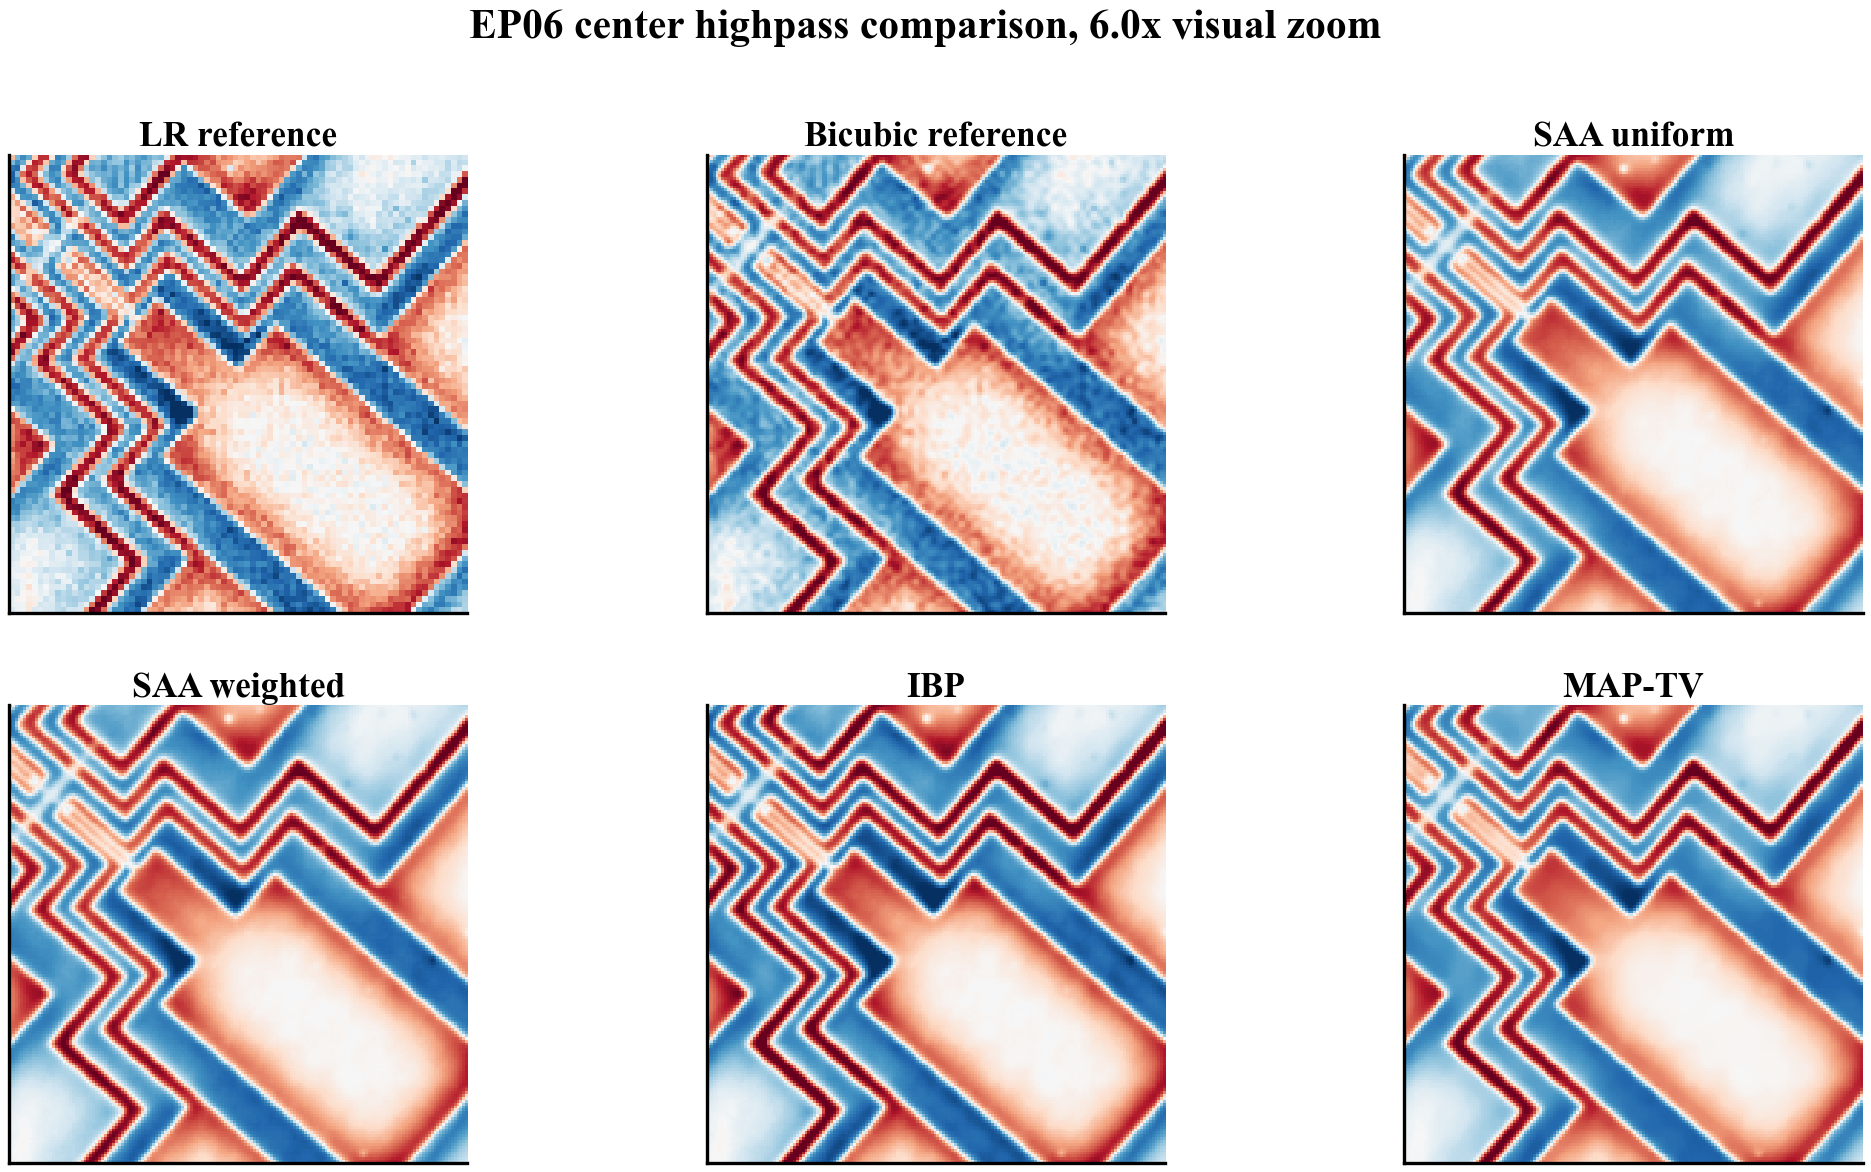
\includegraphics[width=\linewidth]{../figures/ep06_main_comparison.png}
\caption{EP06 center highpass comparison. The figure is a structure-map
visualization, not an absolute temperature image.}
\label{fig:main-comparison}
\end{figure}

\begin{figure}[t]
\centering
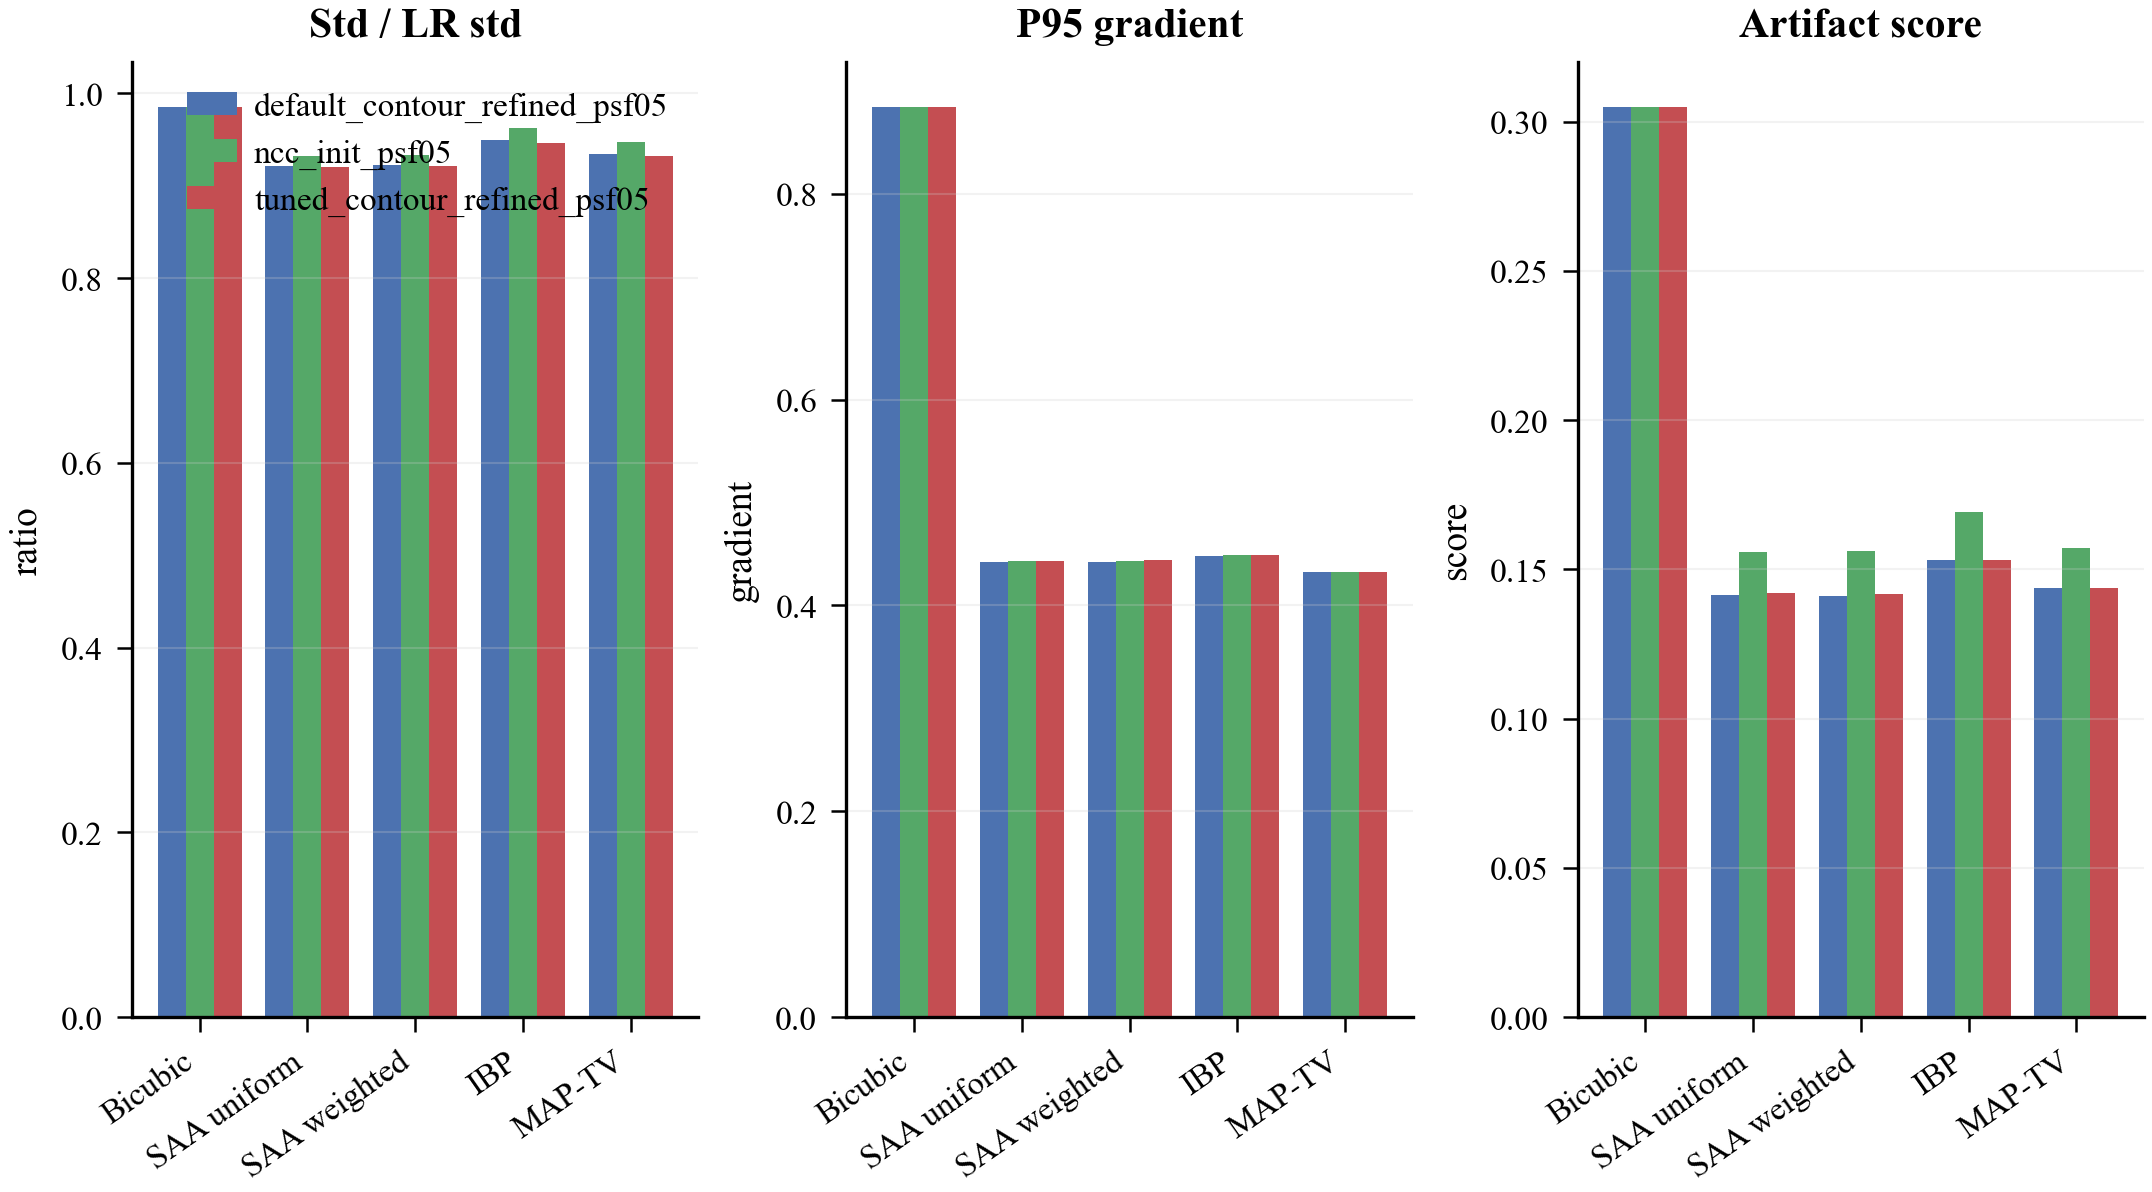
\includegraphics[width=\linewidth]{../figures/ep06_sweep_metrics.png}
\caption{Full alignment sweep metrics for SAA, IBP, and MAP-TV. NCC init raises
artifact risk across the full SR pipeline.}
\label{fig:sweep-metrics}
\end{figure}

The full data-driven alignment sweep contains three experiments:
default contour refined, tuned contour refined, and NCC initialization. All
MAP-TV runs select $\lambda=0.01$ on the highpass track. This consistent
selection of strong regularization is a warning that weakly regularized
forward-model solutions can explain alignment residuals as high-frequency
structure.

\begin{figure}[t]
\centering
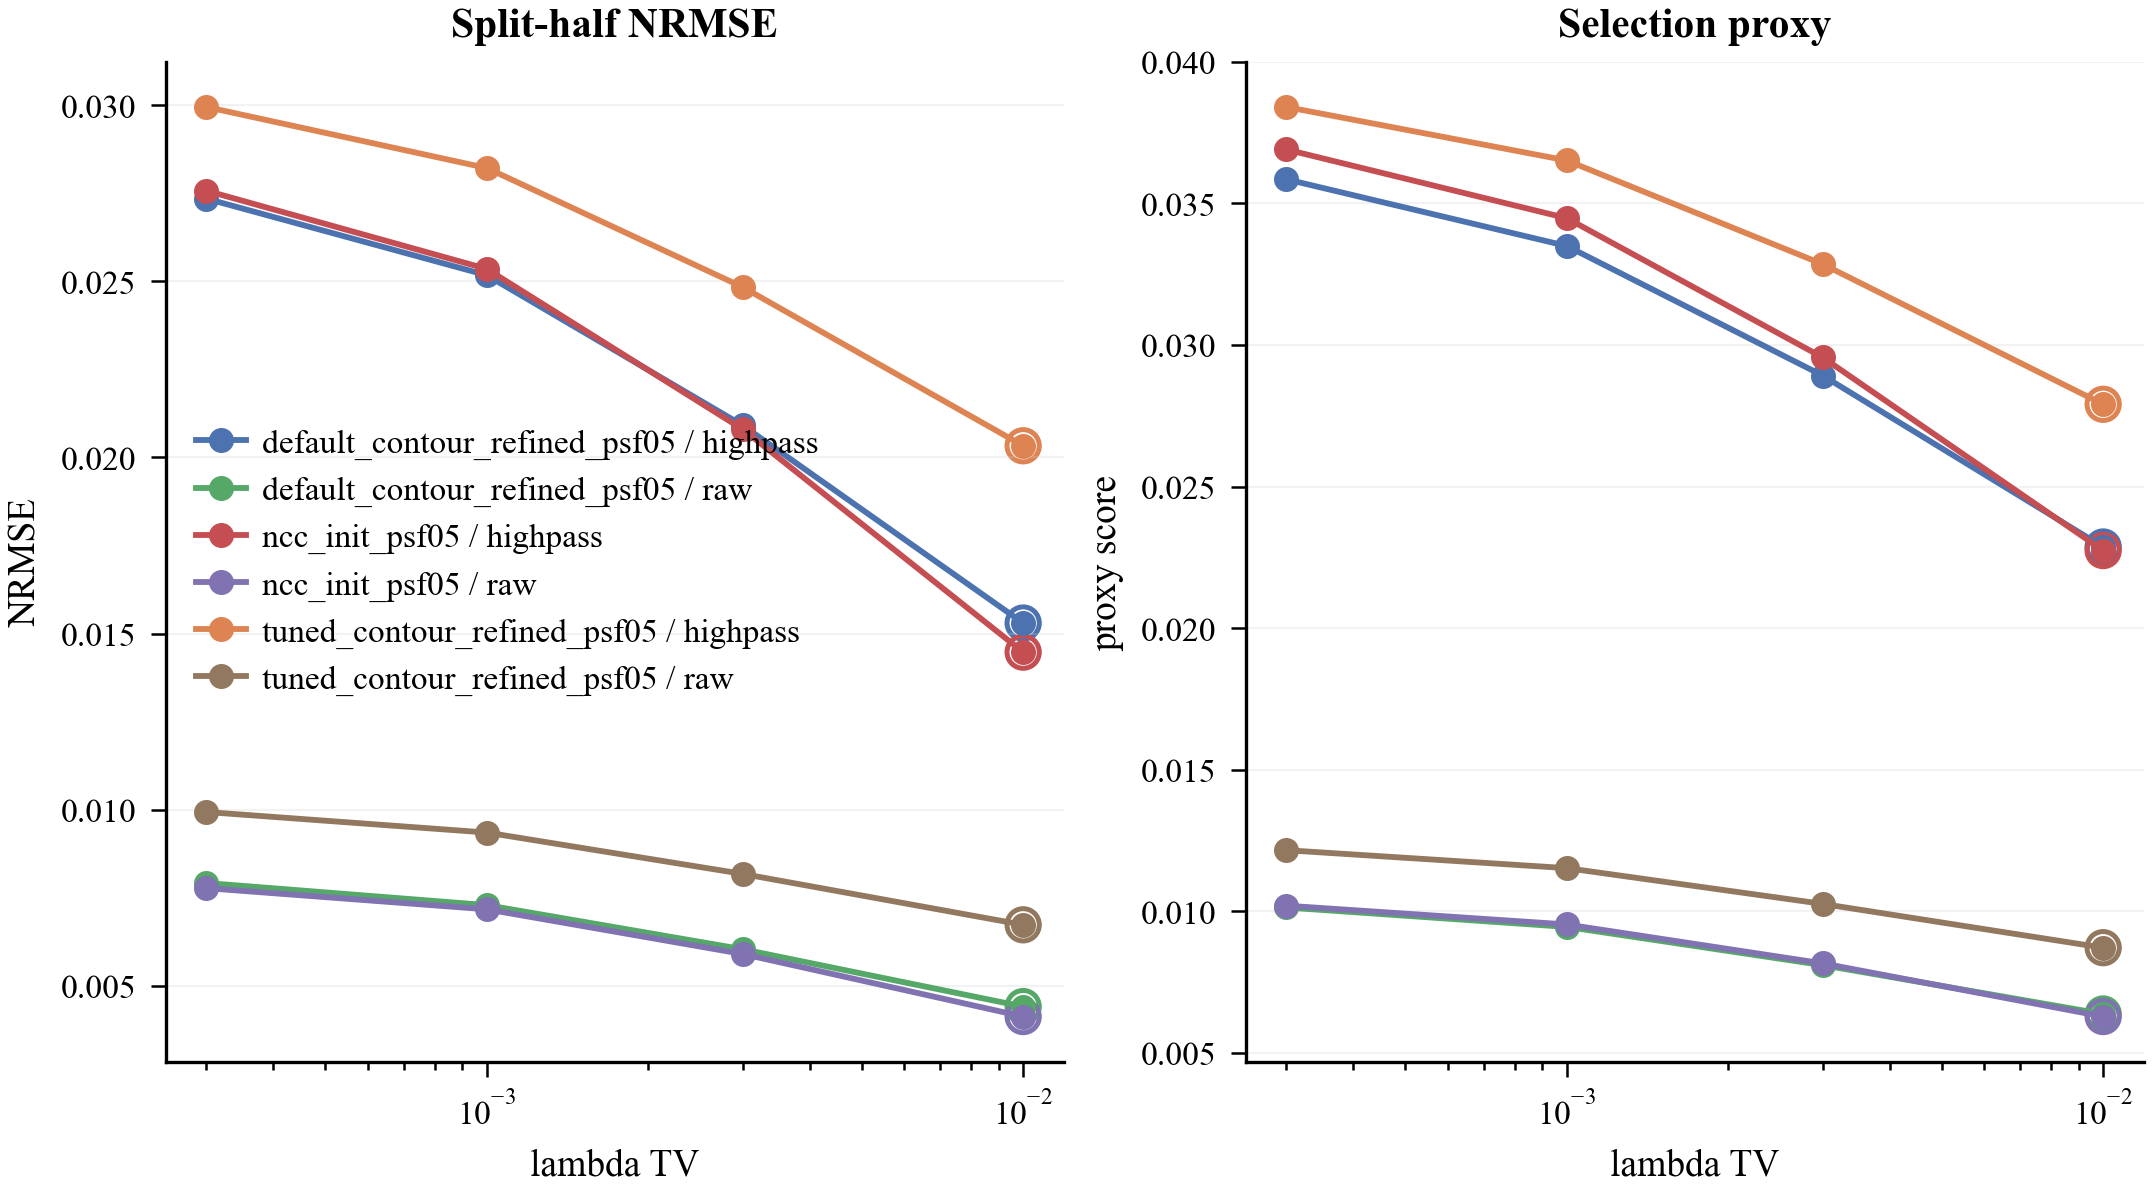
\includegraphics[width=\linewidth]{../figures/ep06_sweep_lambda.png}
\caption{MAP-TV lambda selection under the three alignment variants. Strong
regularization is selected in every case.}
\label{fig:lambda-sweep}
\end{figure}

